% Suggested IEEE text; merge into the report's existing Sections III and IV.
% Requires graphicx and amsmath. Figures span two columns; numbering is report-owned.
\section{Environmental Risk Assessment}
OutdoorWiseSG applies a provisional rule-based environmental assessment to each
catalog route. Rainfall and wind use stations matched to the route start, while
air quality uses curated regional assignments. Numeric WBGT takes precedence over
categorical heat stress, and usable one-hour PM$_{2.5}$ takes precedence over the
rolling 24-hour PSI. Inputs retain their distinct measurement windows.

Component scores use clamped piecewise-linear curves on a 0--100 scale. The
rainfall knots are $(0,0),(1,20),(5,60),(10,100)$ in mm per five minutes;
WBGT knots are $(26,0),(31,50),(33,80),(35,100)$ in degrees Celsius;
PM$_{2.5}$ knots are $(0,0),(55,25),(150,60),(250,85),(350,100)$ in
$\mu$g/m$^3$; and PSI knots are $(0,0),(50,15),(100,35),(200,70),
(300,90),(400,100)$. With usable components, total risk is
\begin{equation}
R=\operatorname{round}_{2}(0.35r+0.35h+0.25a+0.05w).
\end{equation}
Wind scoring is neutral by default ($w=0$), but usable wind evidence is still
required. Missing components are not replaced with zero or renormalized. The
default maximum total is consequently 95. Categorical heat fallback scores
Low/Moderate/High as 20/60/90.

The assessor rechecks availability and observation age at evaluation. Freshness
limits are 15 minutes for rainfall/wind, 45 minutes for WBGT and 120 minutes for
PM$_{2.5}$/PSI. Future availability timestamps and incompatible measurement
contracts cannot contribute. Station estimates beyond 5 km and through the
configured 15 km matching limit are approximate and explicitly flagged.
Incomplete assessments are unknown. Complete assessments become caution at total
risk at least 40, selected component risk at least 70, coarse fallback, or other
configured uncertainty conditions. No hard-block rules are enabled in the default
configuration; supported operator-configured blocks would take precedence even
over an incomplete aggregate. Eligibility does not establish clinical safety.

For complete nonblocked candidates, environmental suitability $E=100-R$ enters
the recommendation score alongside relative distance match $D$, accessibility $A$
and difficulty match $F$:
\begin{align}
D&=100\max(0,1-|d-T|/T),\\
A&=\max(0,100-2a),\\
F&=100\max(0,1-|g-t|/4),\\
S&=\operatorname{round}_{2}(0.45E+0.25D+0.15A+0.15F).
\end{align}
Here $d,T$ are route and target distances, $a$ is straight-line access distance,
and $g,t$ are predicted and target difficulty. With no user location, $A=50$.
Complete eligible/caution candidates share descending score order, with original
baseline rank and route ID resolving ties. Unknown assessments follow as
non-environmental discovery results with null weighted scores; explicit blocks
are excluded.

\section{Evaluation}
\subsection{Environmental Risk and Eligibility Evaluation}
We evaluated the actual scoring interfaces offline without API requests or
changes to production rules. Controlled observations for a fixed catalog route
varied rainfall, WBGT, PM$_{2.5}$ and PSI independently, including curve knots and
policy boundaries. The selected-input branches were nondecreasing and saturated
at their final knots. PSI had no scoring effect while PM$_{2.5}$ was usable,
consistent with the fallback design. These checks concern deterministic rule
behavior rather than physical independence or predictive validity.

All 75 explicit boundary cases met their expected policy outputs. Cases covered
observed zero, missing/stale/future data, inclusive freshness limits, fallback,
spatial support and inclusive blocking under labelled synthetic in-memory rules.
The synthetic blocking thresholds are test fixtures, not deployed safety limits.
Saturated values under the default policy produced caution rather than a block;
missing neutral wind still produced unknown aggregate risk. Rounding before
thresholding can promote a value immediately below 40 to caution.

\begin{figure*}[t]
\centering
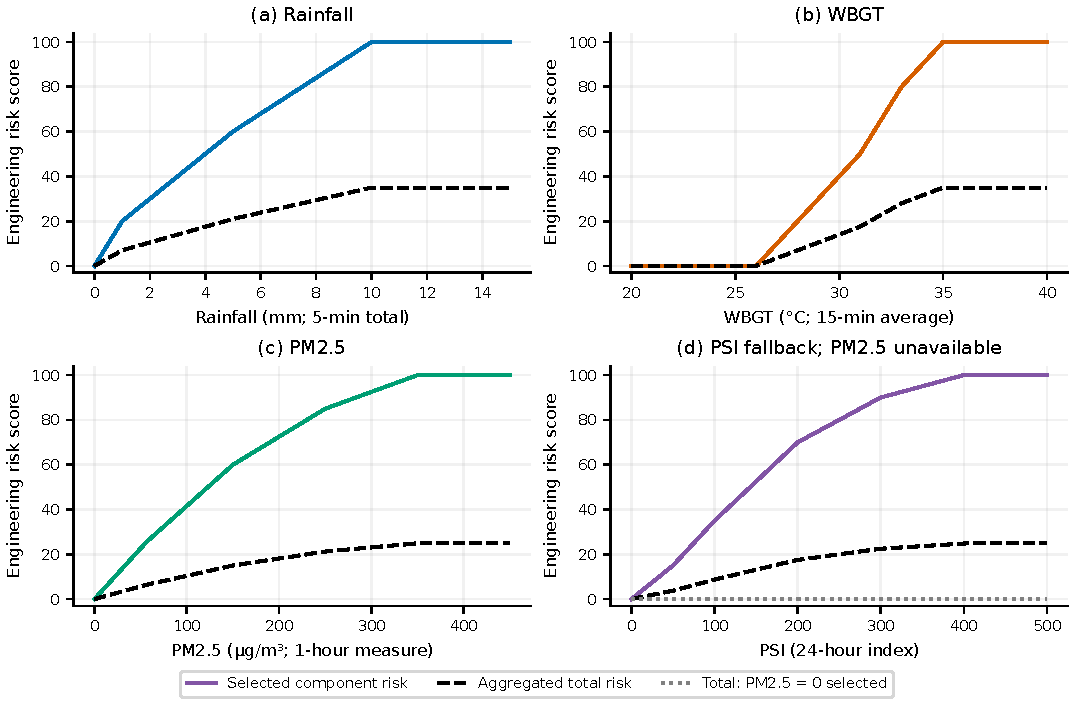
\includegraphics[width=\textwidth]{analysis/risk_model/figure_1_risk_sensitivity.pdf}
\caption{Controlled environmental risk sensitivity. Colored curves show selected
component scores; dashed curves show weighted totals with other selected component
risks held at zero. PSI contributes only when PM$_{2.5}$ is unavailable. These
curves describe provisional rules, not clinically validated response functions.}
\label{fig:risk-sensitivity}
\end{figure*}

\subsection{Catalog Recommendation Evaluation}
We compared all 12 catalog routes using target distance 5 km, target difficulty 3,
no user location, no forecast, identical eligibility rules and identical generic
difficulty estimates. Baselines were distance-only order and the implemented score
with its explicit environmental term disabled and other weights proportionally
rescaled. The latter still includes environment-dependent generic difficulty.
Three archived as-of snapshots were reconstructed using revision availability;
a fourth, explicitly controlled heterogeneous scenario tested ranking sensitivity.
The original October 9 and 10 noon snapshots were retained, each with 12 complete
assessments (5 eligible, 7 caution, none blocked or unknown). No replacement dates
were selected to strengthen the ranking effect. October 15 is a separate
missing-data negative control, rather than primary ranking evidence.
Two routes on October 9 and one on October 10 have very-low confidence from
approximate station inputs; complete scoring does not establish route-wide coverage.

At noon SGT on October 9, 2026, full ranking replaced Bishan--AMK with West Coast
in the Top-3, retaining Pasir Ris Park and Botanic Gardens. Mean reported Top-3
risk changed from 29.47 for both baselines to 25.99. Corresponding mean WBGT was
30.13 versus 29.53 degrees Celsius and PM$_{2.5}$ was 147.33 versus
135.33 $\mu$g/m$^3$; rainfall was zero in both sets. At noon on October 10,
Top-3 membership and mean risk (28.84) were unchanged, although order differed.
Full ranking changed 8 and 6 of the 12 route positions relative to distance-only
ranking on October 9 and 10, respectively; the environmental-term ablation changed
6 and 4 positions. These are deterministic ranking differences, not safety outcomes.
At noon on October 15, rainfall, wind and heat inputs were stale for all routes;
all aggregate scores remained unknown and the methods returned the same discovery
order despite usable air-quality inputs. Rainfall was 30 minutes old against its
15-minute limit, wind 21 against 15, and WBGT 60 against 45. The selected acquisitions
were present and had aged past their limits.
The API/UI disclose unknown assessment and fallback instead of reporting zero risk.

Environmental recommendation weights 0.30 and 0.60, compared with default 0.45,
retained two or three default Top-3 members in the two assessed archived snapshots.
The deliberately heterogeneous fixture changed Top-3 membership substantially,
but does not estimate real-world benefit. Choosing routes using an internal risk
score and then observing lower internal risk is expected; it is not external
evidence of safer outcomes or optimal weights.

\begin{figure*}[t]
\centering
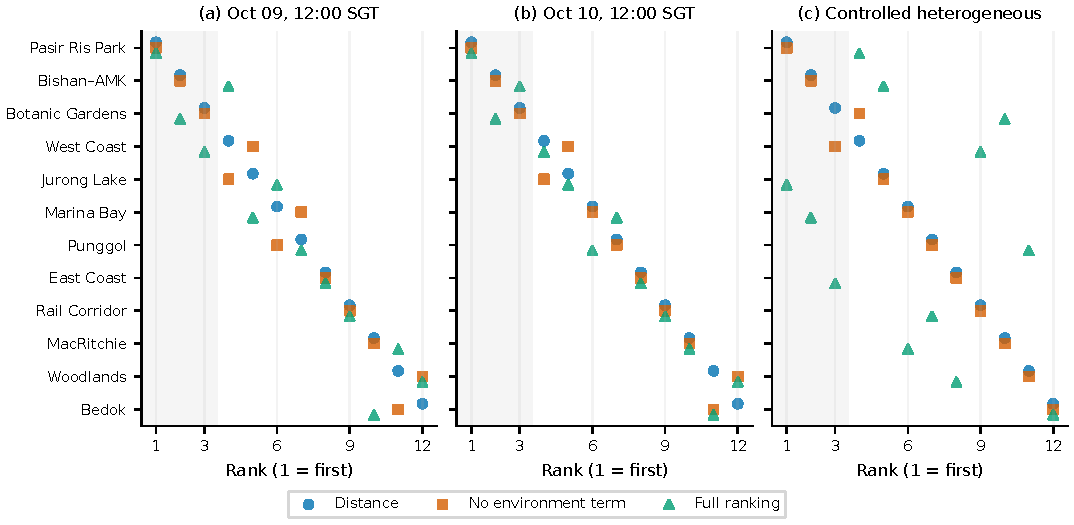
\includegraphics[width=\textwidth]{analysis/risk_model/figure_2_ranking_comparison.pdf}
\caption{Ranking positions for the same 12 catalog routes under three methods.
Shading marks the Top-3. Archived panels use noon Singapore time on October 9
and 10, 2026; the third panel is controlled. Route order is shared across panels.
Small vertical offsets distinguish coincident methods and have no numerical
meaning. October 15 is a separate aggregate-unknown negative control.}
\label{fig:catalog-ranking}
\end{figure*}

\begin{table}[t]
\centering
\caption{October 15 noon SGT negative control: all 12 aggregate risks unknown.}
\label{tab:unknown-control}
\begin{tabular}{lrrl}
\hline
Input & Age (min) & Limit (min) & State\\
\hline
Rainfall & 30 & 15 & Stale\\
Wind & 21 & 15 & Stale\\
WBGT/category & 60 & 45 & Stale\\
PM$_{2.5}$/PSI & 60 & 120 & Usable\\
\hline
\end{tabular}
\end{table}

\subsection{Limitations}
This is rule conformance and descriptive ranking evaluation, not supervised
classification. It uses no external safety outcomes or user-utility ground truth.
Three selected historical times cannot establish representative performance.
Local collection was intermittent, and retrospective matching uses current catalog,
configuration and station metadata. Start-point stations and coarse regions do
not establish route-wide conditions. Generic difficulty consumes raw values
without an independent freshness check. Provisional curves, weights and confidence
bands require external validation before stronger safety or effectiveness claims.

\subsection{Environmental Collection Reliability}
Historical coverage depends both on upstream observation availability and on
operational continuity of the local collector. The retained log contains 11,204
successful and 126 failed source runs, alongside intervals with no completed
polling record. Those intervals do not by themselves identify laptop sleep,
Terminal closure, process termination or provider outages. Some log-supported
active successful polls nevertheless returned demonstrably old observations,
showing that retrieval success alone does not establish measurement recency.
An optional per-user launchd configuration supervises the existing CSV collector
independently of Terminal, with additive process/source diagnostics and the existing
single-worker lease. Recovery was checked using isolated fixtures, not sleep or
native launchd activation. Local supervision cannot collect during sleep, logout
or power-off; uninterrupted collection requires an always-on connected host.
